\documentclass{article}
\usepackage{listings}
\usepackage{xcolor}
\usepackage{graphicx}

\definecolor{dkgreen}{rgb}{0,0.6,0}
\definecolor{gray}{rgb}{0.5,0.5,0.5}
\definecolor{mauve}{rgb}{0.58,0,0.82}
\definecolor{orange}{rgb}{1.0,0.5,0}

\lstset{frame=tb,
  language=Java,
  aboveskip=3mm,
  belowskip=3mm,
  showstringspaces=false,
  columns=flexible,
  basicstyle={\small\ttfamily},
  numbers=none,
  numberstyle=\color{orange},
  keywordstyle=\color{blue},
  commentstyle=\color{dkgreen},
  stringstyle=\color{mauve},
  breaklines=true,
  breakatwhitespace=true,
  tabsize=3
}

\title{Analysis of Poisson Relaxation with Threads}
\date{\today}
\author{Arthur Ceccotti - 8544173}

\begin{document}
\maketitle

\section{Introduction}
I have written a version of the \textit{Poisson's Equation} using the relaxation technique with a variable number of threads. Correctness of the program was guaranteed by checking the expected number of iterations (65,251) and also manually visualizing the array convergence over different iterations, as seen in figure \ref{fig:iterations}, produced from listings \ref{lst:plot} and \ref{lst:run}.

\begin{figure}
\label{fig:iterations}
\caption{Approximation of Poisson's Equation over different iterations}
\centering
\begin{minipage}{0.45\textwidth}
  \centering
  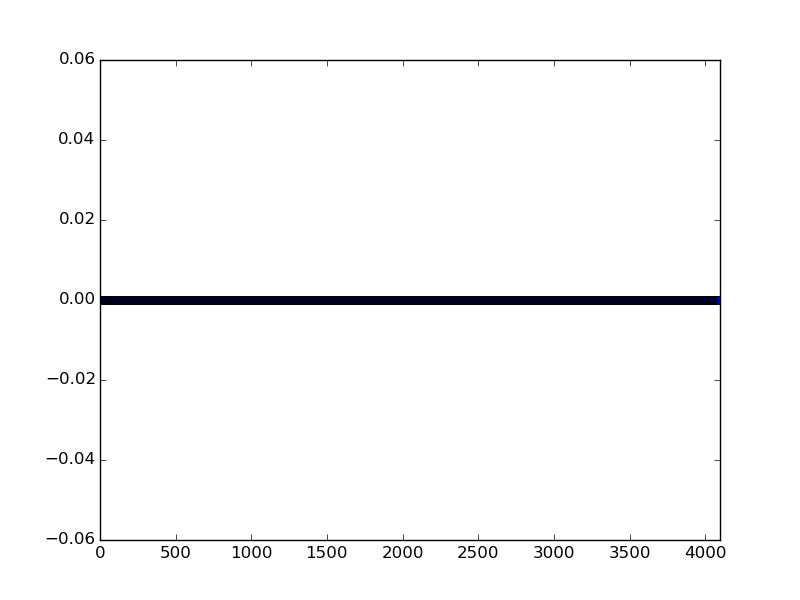
\includegraphics[width=1\linewidth, natwidth=800, natheight=600]{graphs/it1.png}\\
  0 iterations
\end{minipage}
\begin{minipage}{0.45\textwidth}
  \centering
  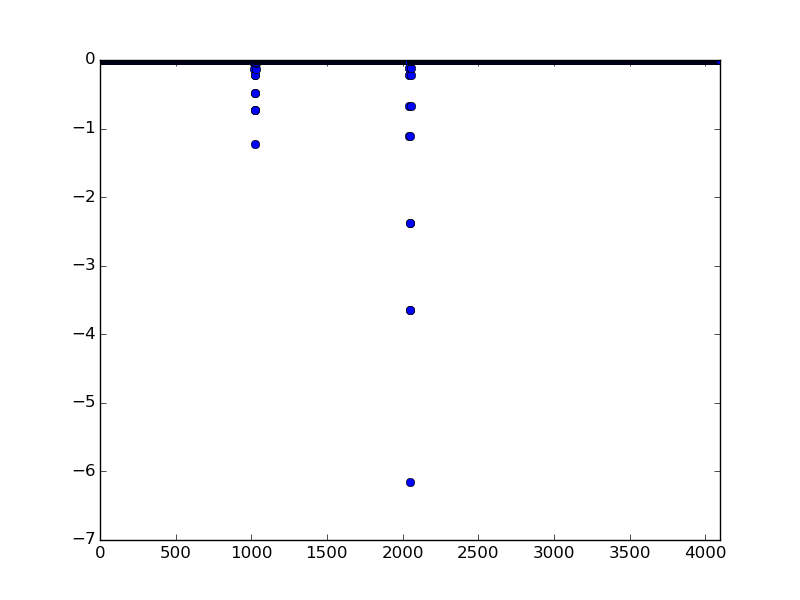
\includegraphics[width=1\linewidth, natwidth=800, natheight=600]{graphs/it10.png}\\
  10 iterations
\end{minipage}
\begin{minipage}{0.45\textwidth}
  \centering
  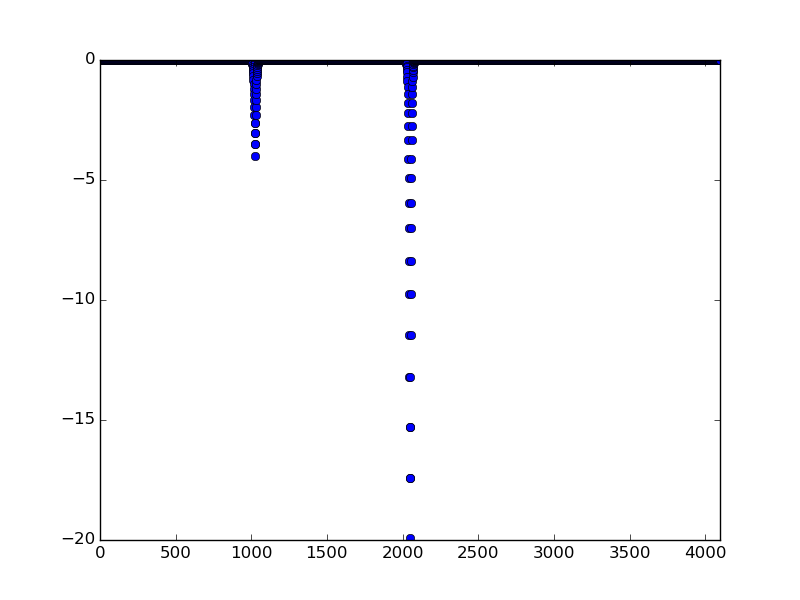
\includegraphics[width=1\linewidth, natwidth=800, natheight=600]{graphs/it100.png}\\
  100 iterations
\end{minipage}
\begin{minipage}{0.45\textwidth}
  \centering
  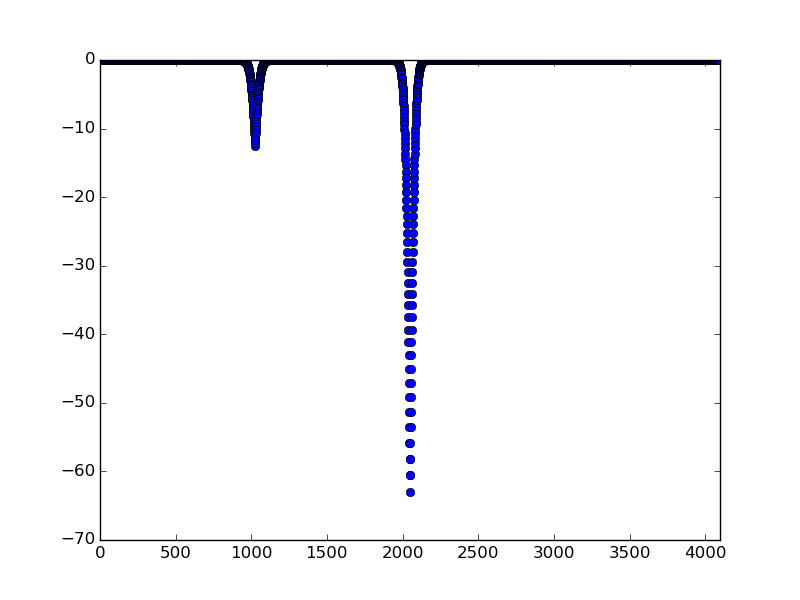
\includegraphics[width=1\linewidth, natwidth=800, natheight=600]{graphs/it1000.png}\\
  1,000 iterations
\end{minipage}
\begin{minipage}{0.45\textwidth}
  \centering
  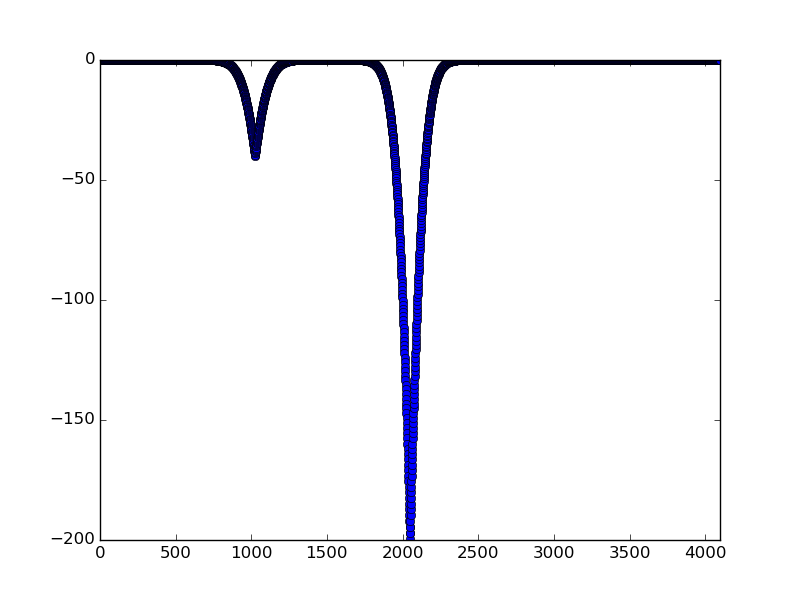
\includegraphics[width=1\linewidth, natwidth=800, natheight=600]{graphs/it10000.png}\\
  10,000 iterations
\end{minipage}
\begin{minipage}{0.45\textwidth}
  \centering
  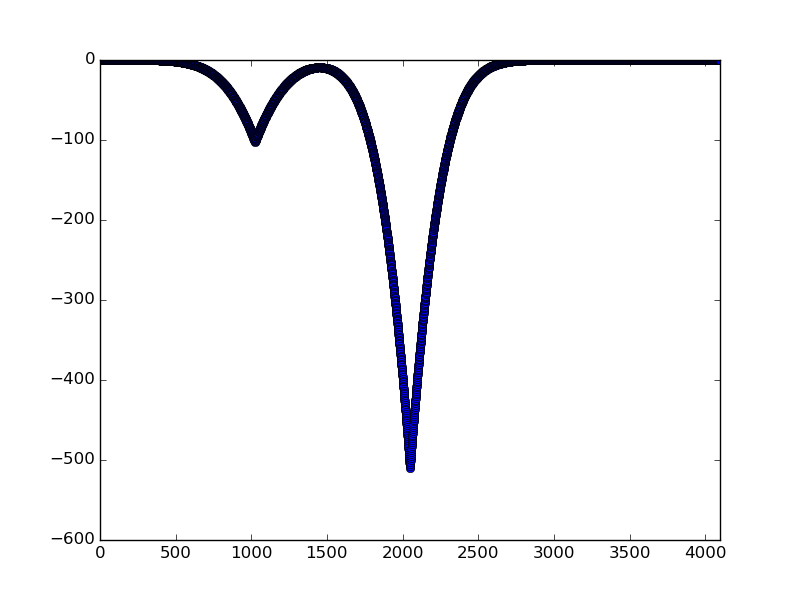
\includegraphics[width=1\linewidth, natwidth=800, natheight=600]{graphs/itFinal.png}\\
  65,250 iterations
\end{minipage}
\end{figure}	

Intermittent performance drops/spikes were reduced by running every instance 10 times on \textit{mcore48.cs.man.ac.uk}\footnote{\label{machinespecs} \\
  Dell/AMD quad 12-core (48 cores total), each with specs:\\
  model name: AMD Opteron(tm) Processor 6174 \\
  clock speed: 2.2 GHZ \\
  cache size: 512 KB \\}, allowing the gathering of average values and standard deviation. The data produced from all the runs was analysed and plotted by a Python script under listing \ref{lst:process}.

\section{Evaluation}

Figure \ref{fig:perf} plots the average performance and error bars (based on standard deviation) of the program for this constant vector size. As can be seen in the figure, the overall performance drops drastically with the addition of new threads, which would be counter intuitive to the advantages of multithreaded programs. I evaluate that the vector size (or accuracy of the problem) is too small (only about 4,000) to allow improvements from multithreading. As mentioned in earlier courseworks, \textbf{thread initialization} is expensive (processor-wise and memory-wise) and so is \textbf{blocking at the join}, meaning for small instances such bottleneck may take longer than a single thread solving the problem by itself, which is exactly the case here.

In this program we need to use a \textbf{CyclicBarrier} to make sure all threads are ready to proceed (avoiding writing to boundary values while they are being read), which highly impacts performance, similarly to the join. I initially wrote a solution in which each thread awaited twice at the barrier at each iteration\footnote{\label{awaittwice} Once to read the region of the array, writting to the \textit{newV} + once to check for convergence and write values back to \textit{V}}, but that introduced even larger bottleneck, as threads were doing very little work before reaching a check-point to wait for other threads. This was improved by passing a Runnable to be executed upon tripping of the barrier, allowing the use of a single await at each iteration (see code at listing \ref{lst:poisson-thread}). The comparison of both implementations is shown in figure \ref{fig:comp-perf}, in which the speedup advantages of using a single await per iteration is clearly visible.

Another enhancement was made by having each thread checking for convergence of their own regions concurrently and if at least one thread had not converged, it would vote to have another iteration, which would be accepted by all threads. This is much faster than having a single thread scanning the whole array, checking for convergence, which completely defeats the purpose of using threads.

Although these enhancement may be barely visible with such a small array (about 4,000 elements), I evaluate that my technique, using \textit{one await per iteration} and \textit{multithreaded convergence check} would perform very well for large vectors.

A factor which could also impact performance is \textbf{cache misses for large problems}, specially given we are using arrays of doubles (64-bit elements). If the working set of a thread cannot always be kept in cache (ie. it is full), cache misses would highly slow down the program. This is very unlikely the case for our current problem, but could impact an array with millions of elements.

\begin{figure}
  \centering
  \caption{Performance plot}
  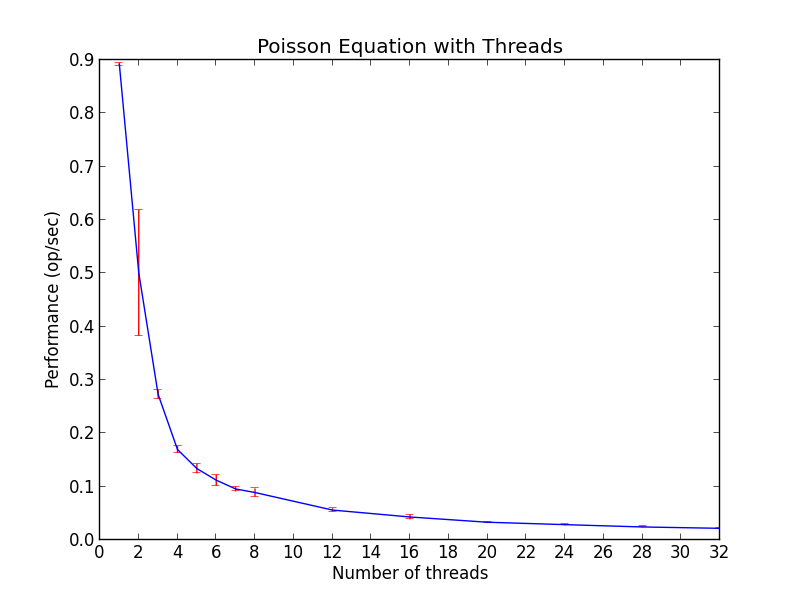
\includegraphics[width=0.8\linewidth, natwidth=800, natheight=600]{graphs/performance.png}
  \label{fig:perf}
\end{figure}

A linear, \textbf{ideal performance} increase with the addition of threads is shown on figure \ref{fig:ideal-perf} which assumes that if one thread runs at 1 op/sec, then two threads will run at 2 op/sec. In summary, for the Poisson's Equation problem, as mentioned earlier, this O(\textit{n}) speedup is surely not realistic due to the following multithreading bottlenecks:

\begin{itemize}
\setlength\itemsep{0.35em}
  \item \textbf{Awaiting at barrier}
  \item \textbf{Final join}
  \item \textbf{Convergence voting}
  \item \textbf{Cache misses for large vectors}
\end{itemize}


\begin{figure}
\centering
\begin{minipage}{0.47\textwidth}
  \centering
  \caption{Performance comparison}
  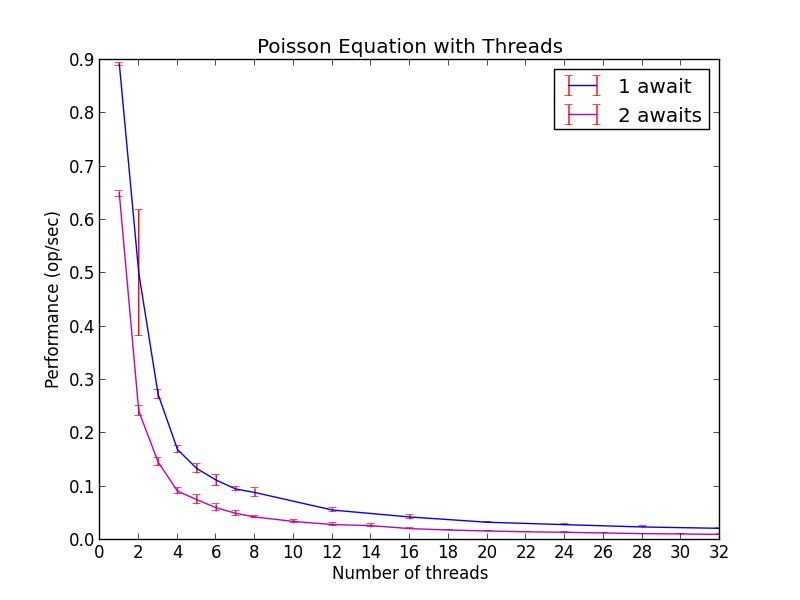
\includegraphics[width=1\linewidth, natwidth=800, natheight=600]{graphs/comparison_performance.png}
  \label{fig:comp-perf}
\end{minipage}
\begin{minipage}{0.47\textwidth}
  \centering
  \caption{Ideal performance}
  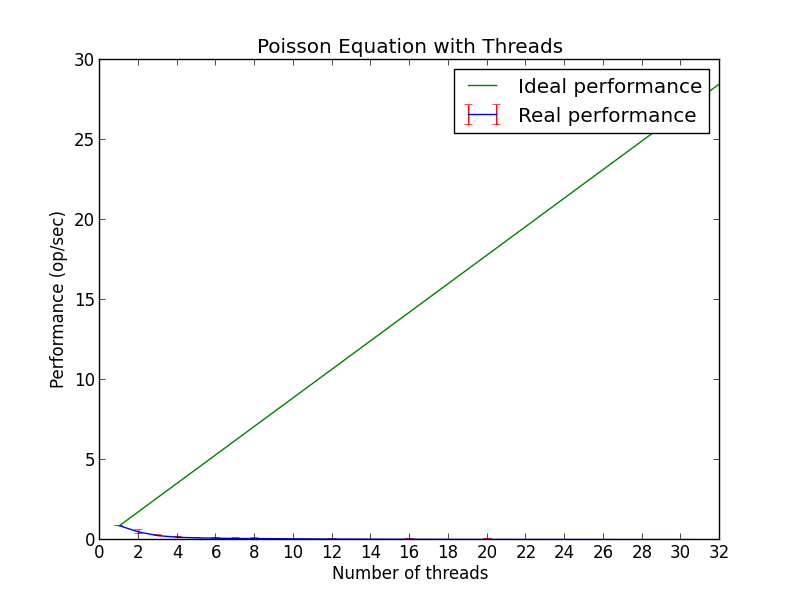
\includegraphics[width=1\linewidth, natwidth=800, natheight=600]{graphs/ideal_performance.png}
  \label{fig:ideal-perf}
\end{minipage}
\end{figure}

\clearpage
\section{Code}
  \subsection{Poisson Solver}
    \lstinputlisting[language=Java,
                     caption=Poisson Solver,
                     label={lst:poisson-solver}]{src/PoissonSolver.java}

    \lstinputlisting[language=Java,
                     caption=Array Wrapper,
                     label={lst:array-wrapper}]{src/ArrayWrapper.java}

    \lstinputlisting[language=Java,
                     caption=Poisson Thread,
                     label={lst:poisson-thread}]{src/PoissonThread.java}

  \subsection{Data Evaluation Scripts}  
    \lstinputlisting[language=bash,
                     caption=Bash scripts to run PoissonThreads with multiple parameters,
                     label={lst:bashscripts}]{src/DemoTuca.sct}

    \lstinputlisting[language=Python,
                     caption=Python scripts to gather and plot results,
                     label={lst:process}]{src/process.py}

    \lstinputlisting[language=bash,
                     caption=Bash scripts to plot convergence over iterations,
                     label={lst:run}]{run}

    \lstinputlisting[language=Python,
                     caption=Python scripts to plot convergence over iterations,
                     label={lst:plot}]{plot.py}
\end{document}